\documentclass{article}
\usepackage[spanish]{babel}
\usepackage[numbers,sort&compress]{natbib}
\usepackage[T1]{fontenc}
\usepackage[ansinew]{inputenc}
\usepackage{graphicx}
\usepackage{url}
\usepackage{caption}
\usepackage{float}
\usepackage{subcaption}
\usepackage{caption}
\usepackage{listings}
\usepackage{amsmath}
\usepackage{natbib}



\title {Algoritmo gen\'etico}
\author{Oscar Qui\~nonez}

\begin{document}

\maketitle
 
\section{Objetivo}\label{met}

Se plantea un problema conocido como ``el problema de la mochila'' en el que se debe regular la cantidad de objetos que se colocan dentro de ella, debido a que tiene una capacidad limitada en cuesti\'on de peso, en base a este problema, se busca realizar una simulaci\'on de un algoritmo gen\'etico el cual se var\'ia la selecci\'on de los padres de la manera conocida como ``ruleta'' \cite{satuelisa}.  

\section{Metodolog\'ia}\label{met}

En esta simulaci\'on fue necesario el uso del programa Python 3.7 en el que se tom\'o como c\'odigo base el proporcionado durante la clase \cite{doctora} para posteriormente plantear 3 escenarios posibles: 1) el valor y el peso son independientes entre ellos, 2) el valor y el peso est\'an relacionados entre ellos y 3) el peso es independiente pero el valor es inversamente proporcional a este.
Al variar la selecci\'on de padres a tipo ``ruleta'', cada uno ten\'ia una probabilidad de ser tomado en cuenta, y al tomar los 3 criterios anteriormente planteados, se puede determinar el valor del algoritmo gen\'etico y compararlo con el algoritmo exacto. Los valores de n usados en esta simulaci\'on fueron 100, 200, 300 y 400.


\section{Resultados y Discusi\'on}\label{res}

Al ejecutar el c\'odigo con las variaciones mencionadas se obtuvieron primeramente las gr\'aficas que nos indican la diferencia de los valores al usar o no usar la ruleta, estas gr\'aficas se pueden apreciar en la figura 1 que se presenta a continuaci\'on.
En el cuadro1 se muestra los valores obtenidos al variar la cantidad de objetos y se destacan los valores m\'aximos y \'optimos de cada uno, de manera mas representativa se pueden ver las gr\'aficas de estos valores y como var\'ian entre ellos en las figuras 2, 3, 4 y 5.


\begin{figure}[H]
       \centering
       \begin{subfigure}[b]{0.60\linewidth}
           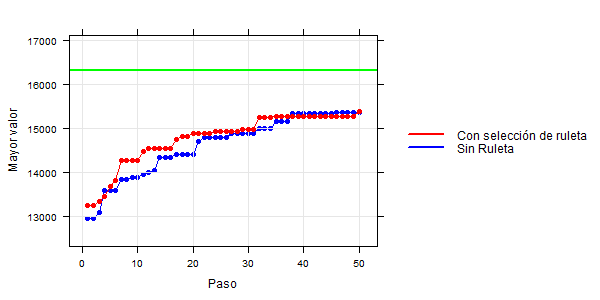
\includegraphics[width=\linewidth]{100tarea10.png}
           \caption{100 objetos}
           \label{fig:westminster_lateral}
        \end{subfigure}
          \begin{subfigure}[b]{0.60\linewidth}
           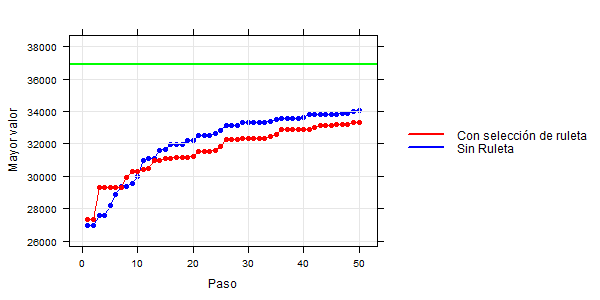
\includegraphics[width=\linewidth]{200tarea10.png}
           \caption{200 objetos}
           \label{fig:westminster_lateral}
        \end{subfigure}    
        \caption{Comparaci\'on de la ruleta con 100 y 200 objetos}
        \label{fig:westminster}
\end{figure}

\begin{table} [H]
 \caption{Tabla de resultados para las distintaas cantidades de n.}
 \label{t1}
 \begin{center}
 \begin{tabular}{rrrrrrr}
\texttt{Objetos} & \texttt{Valor m\'aximo} & \texttt{Valor \'optimo} &\texttt{Instancia} \\
100  & 7326.288381842508 & 75851.55212057414  & 1  \\ 
100  & 68468.98351482986 & 55795.300566274185    & 2\\ 
100  &  51964.798682299166 & 43479.15872730447  & 3  \\ 
200  &15368.983690630148  &13571.3126008619583  & 1  \\ 
200  & 17894.877000934695   &8721.51234211876 & 2 \\ 
200  & 14832.970082181477   & 12135.028209092558 & 3   \\ 
300  & 32763.83926134712 & 21985.93465812870 &  1 \\ 
300  & 28754.157541097403 & 18963.883314069720 & 2  \\ 
400 & 52301.06212532473&21369.348512678901  & 1  \\ 
400 & 42034.773495068867&35991.030450982477  & 2   \\ 
400 & 40782.74748446381& 27004.364789015584  & 3 \\ 


\end{tabular}
\end{center}
\end{table}

\begin{figure}[H]
       \centering
       \begin{subfigure}[b]{0.49\linewidth}
           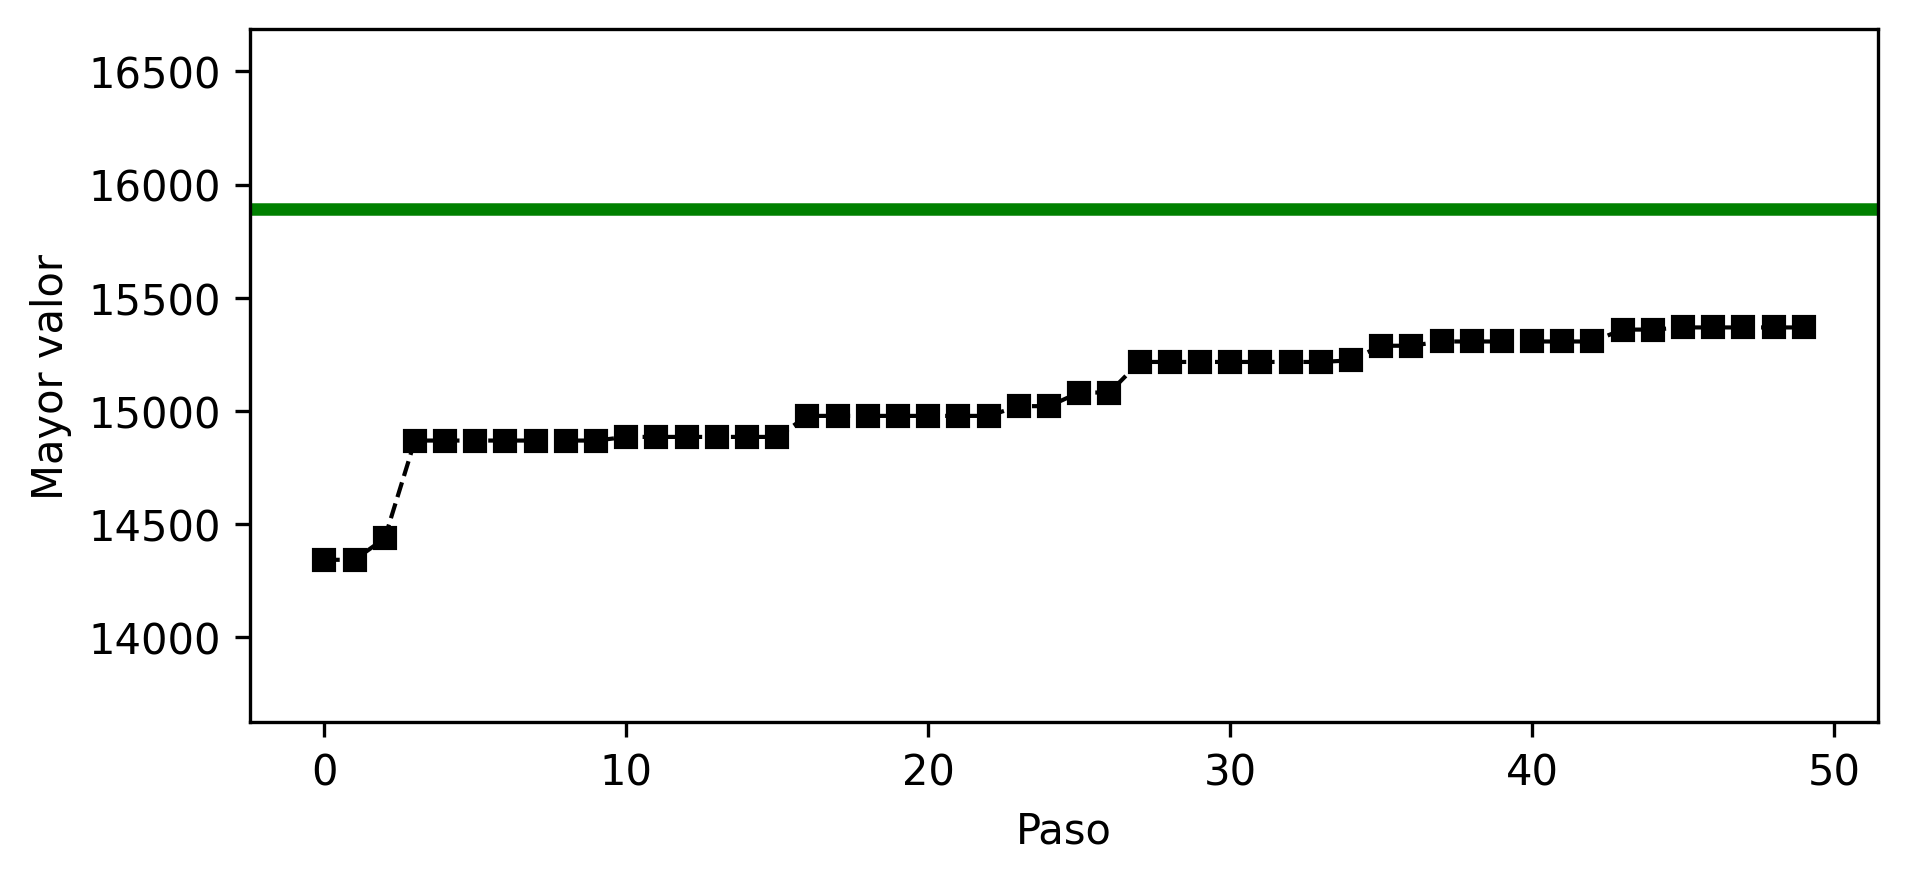
\includegraphics[width=\linewidth]{p100.png}
           \caption{Instancia 1}
           \label{fig:westminster_lateral}
        \end{subfigure}
          \begin{subfigure}[b]{0.49\linewidth}
           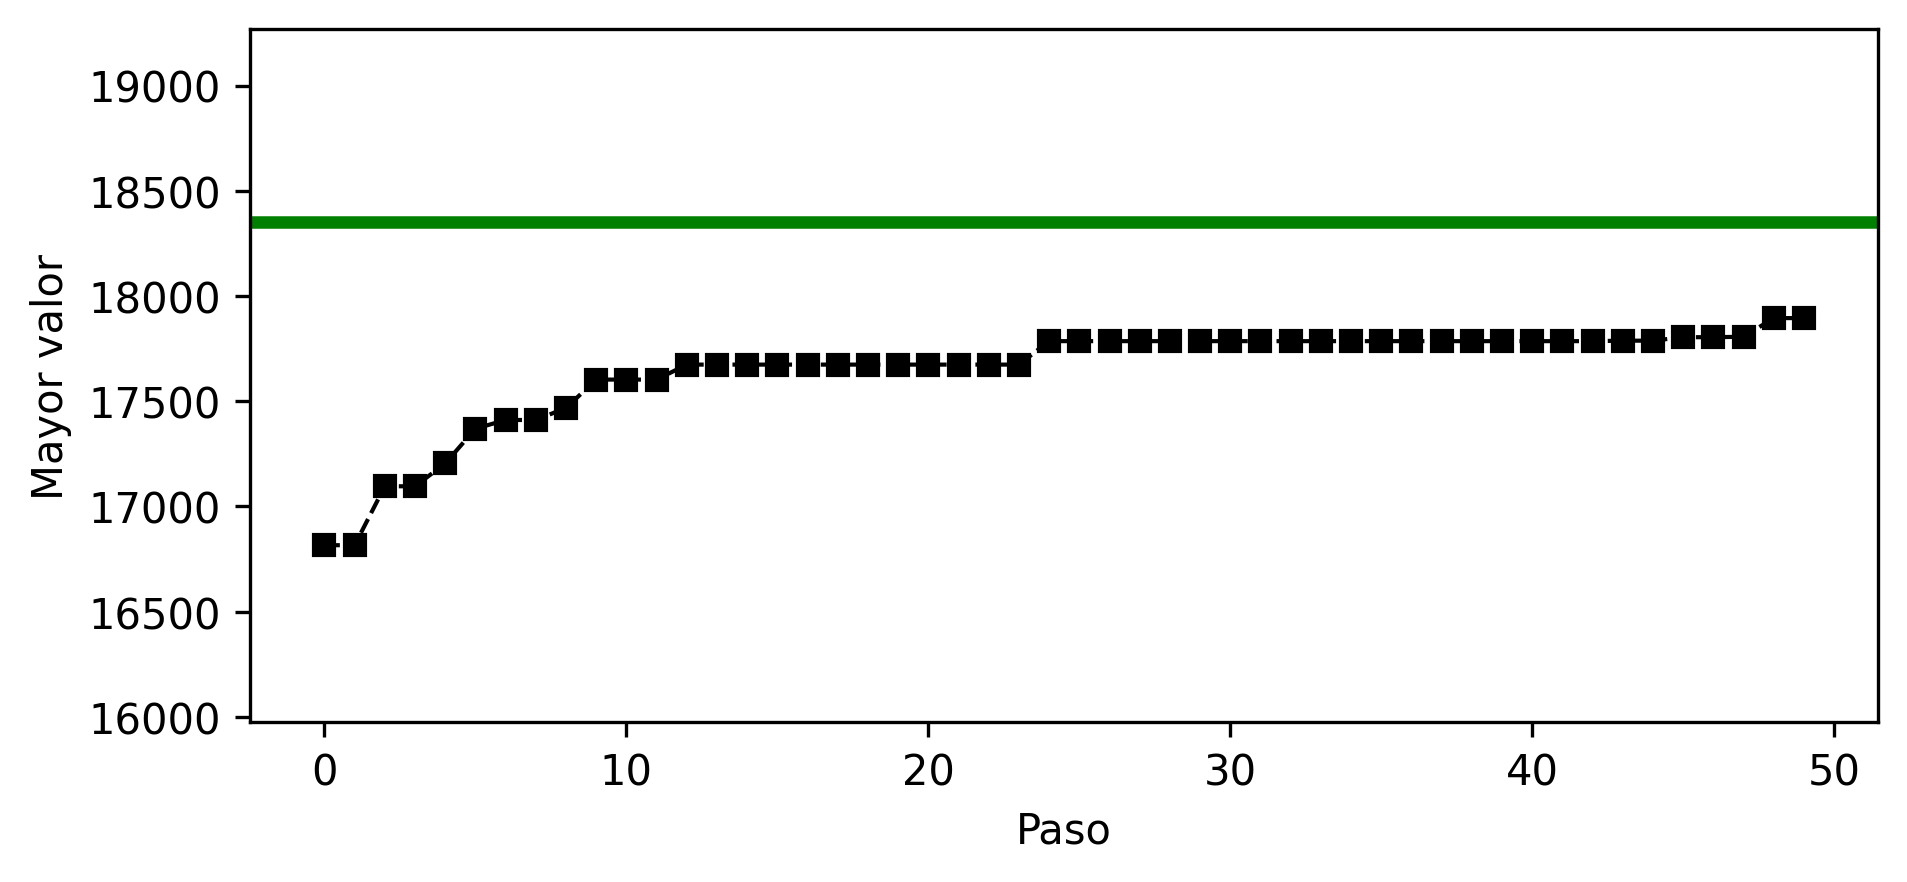
\includegraphics[width=\linewidth]{p100 i 2.png}
           \caption{Instancia 2}
           \label{fig:westminster_lateral}
        \end{subfigure}
       \begin{subfigure}[b]{0.49\linewidth}
           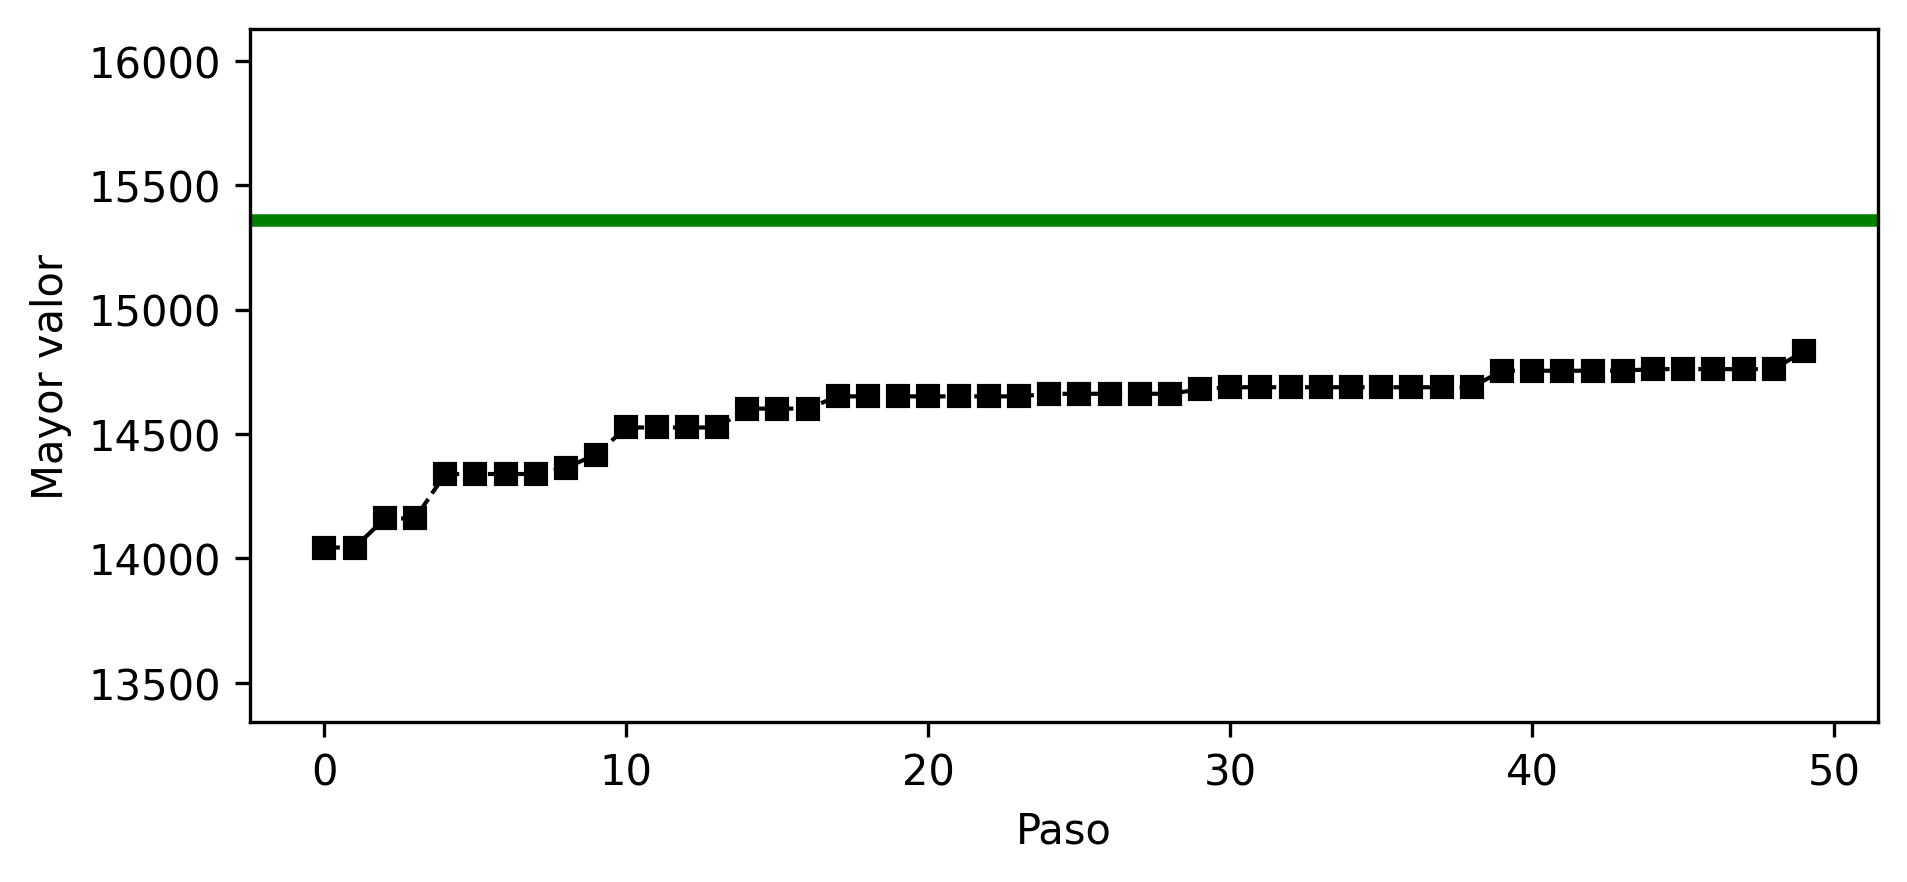
\includegraphics[width=\linewidth]{p100 i 3.png}
           \caption{Instancia 3}
           \label{fig:westminster_lateral}
        \end{subfigure}   
        \caption{3 instancias para n=100}
        \label{fig:westminster}
\end{figure}

\begin{figure}[H]
       \centering
       \begin{subfigure}[b]{0.49\linewidth}
           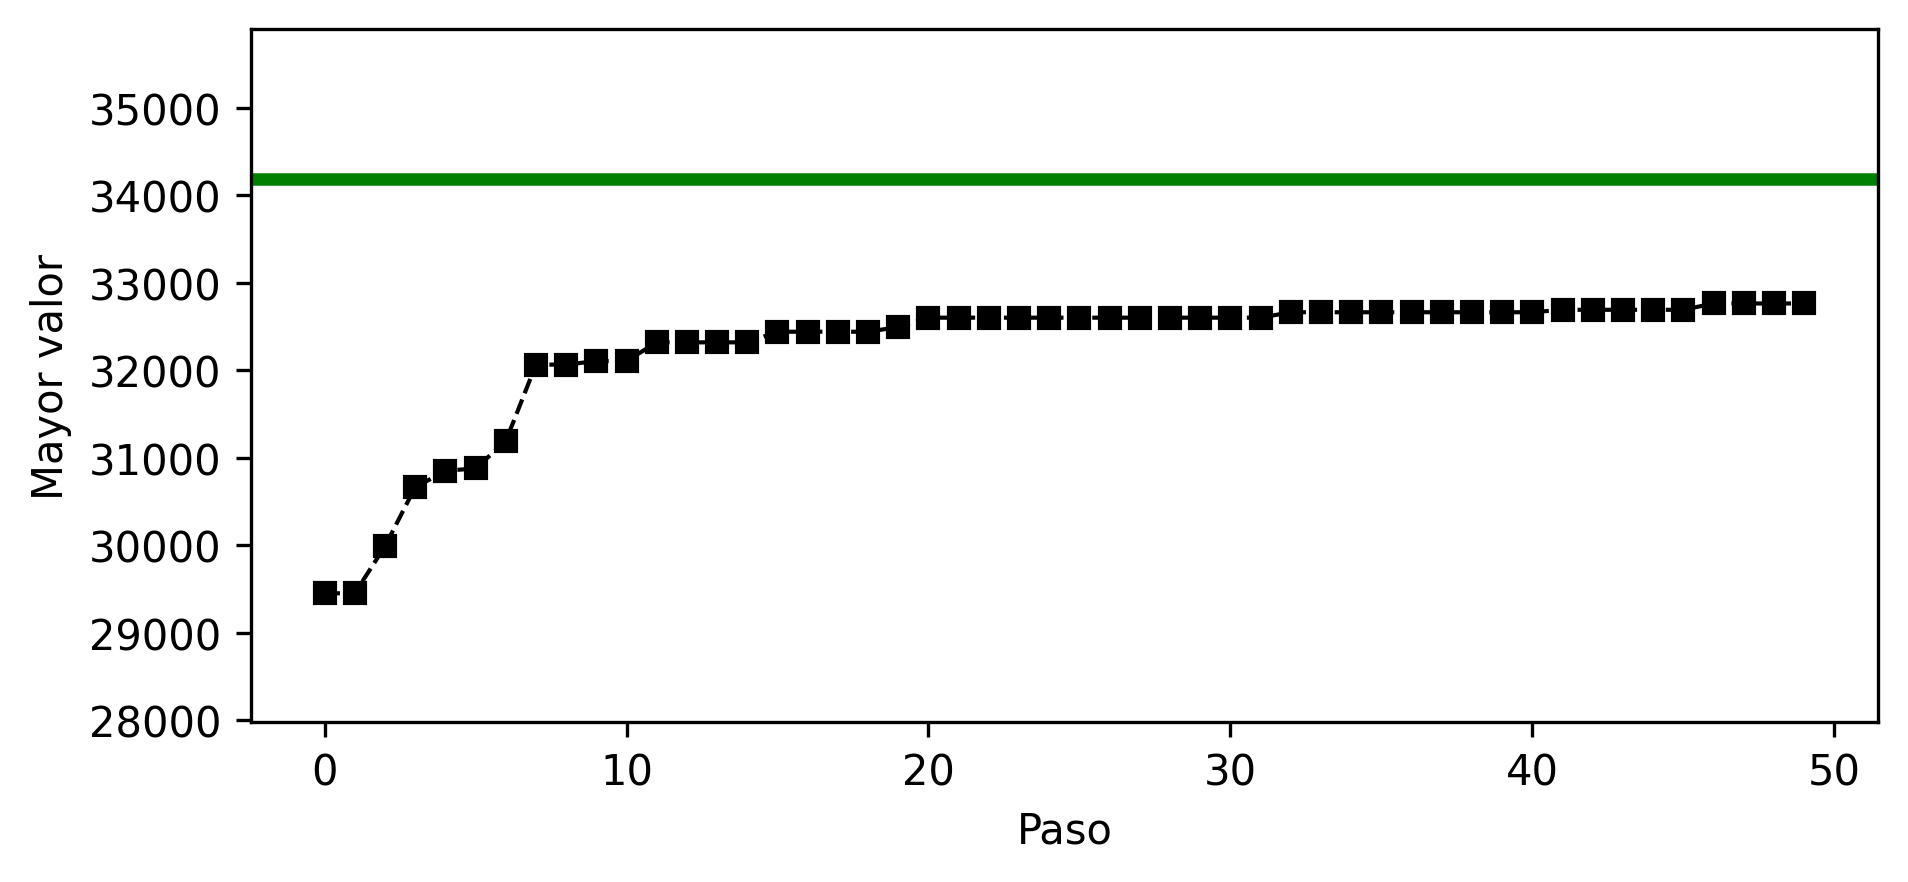
\includegraphics[width=\linewidth]{p200.png}
           \caption{Instancia 1}
           \label{fig:westminster_lateral}
        \end{subfigure}
          \begin{subfigure}[b]{0.49\linewidth}
           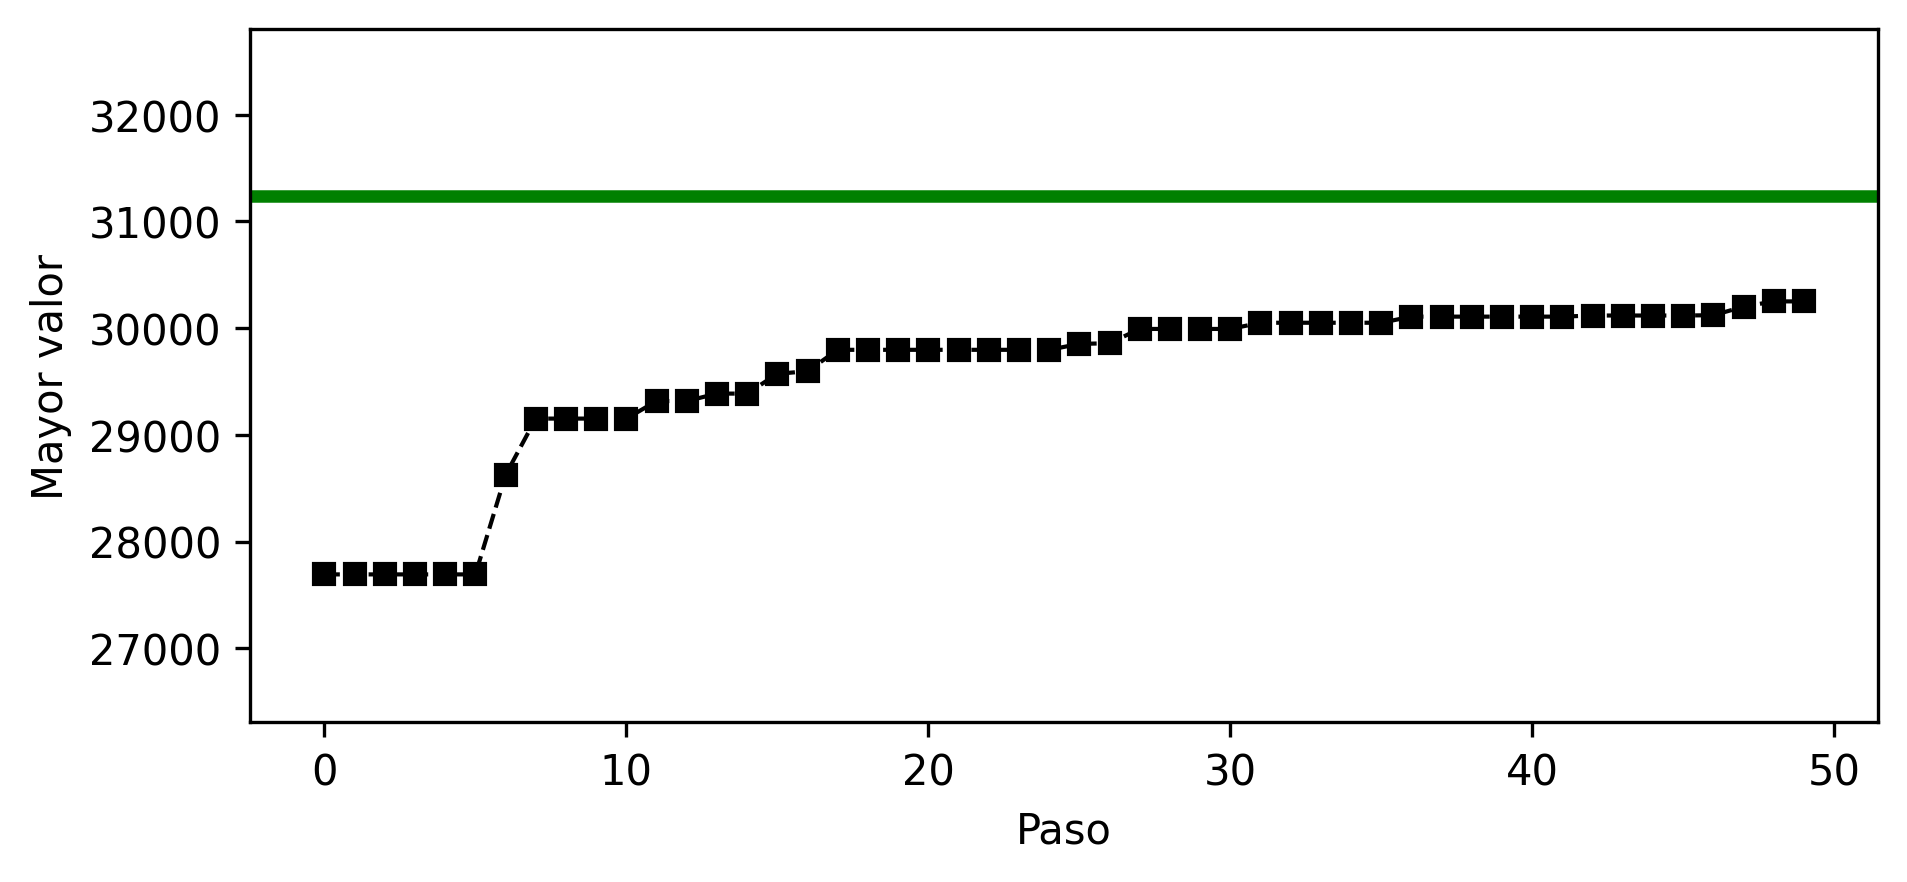
\includegraphics[width=\linewidth]{p200 i 2.png}
           \caption{Instancia 2}
           \label{fig:westminster_lateral}
        \end{subfigure}
       \begin{subfigure}[b]{0.49\linewidth}
           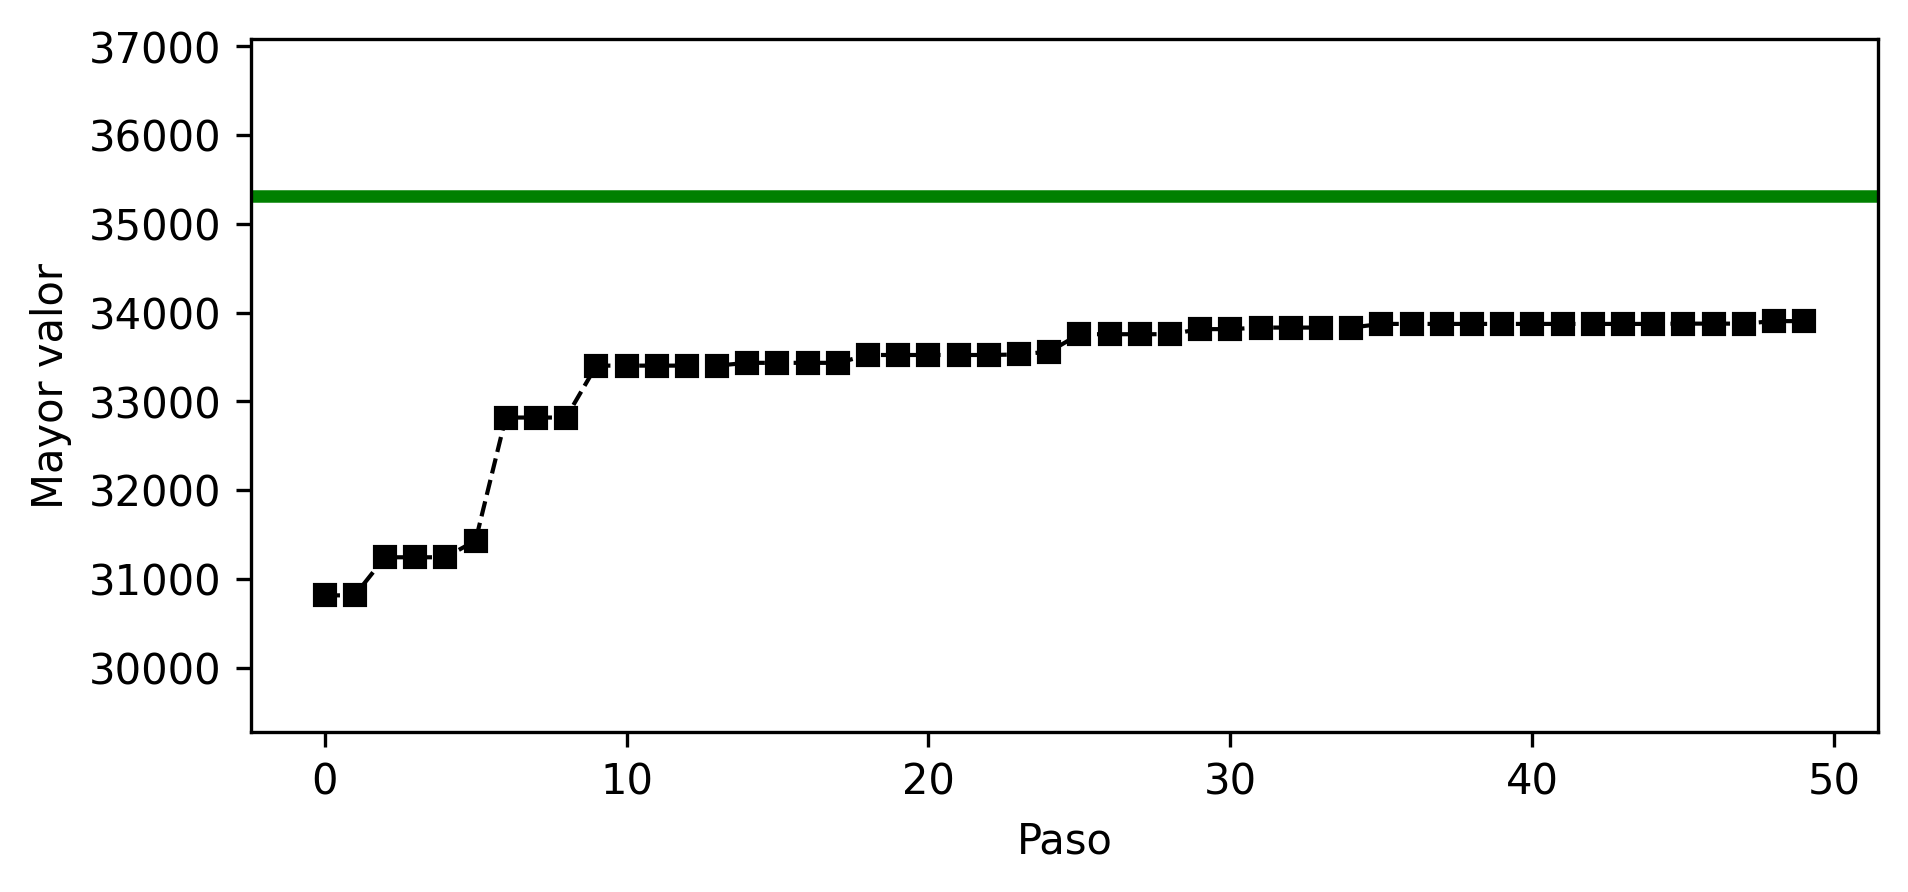
\includegraphics[width=\linewidth]{p200 i 3.png}
           \caption{Instancia 3}
           \label{fig:westminster_lateral}
        \end{subfigure}   
        \caption{3 instancias para n=200}
        \label{fig:westminster}
\end{figure}

\begin{figure}[H]
       \centering
       \begin{subfigure}[b]{0.49\linewidth}
           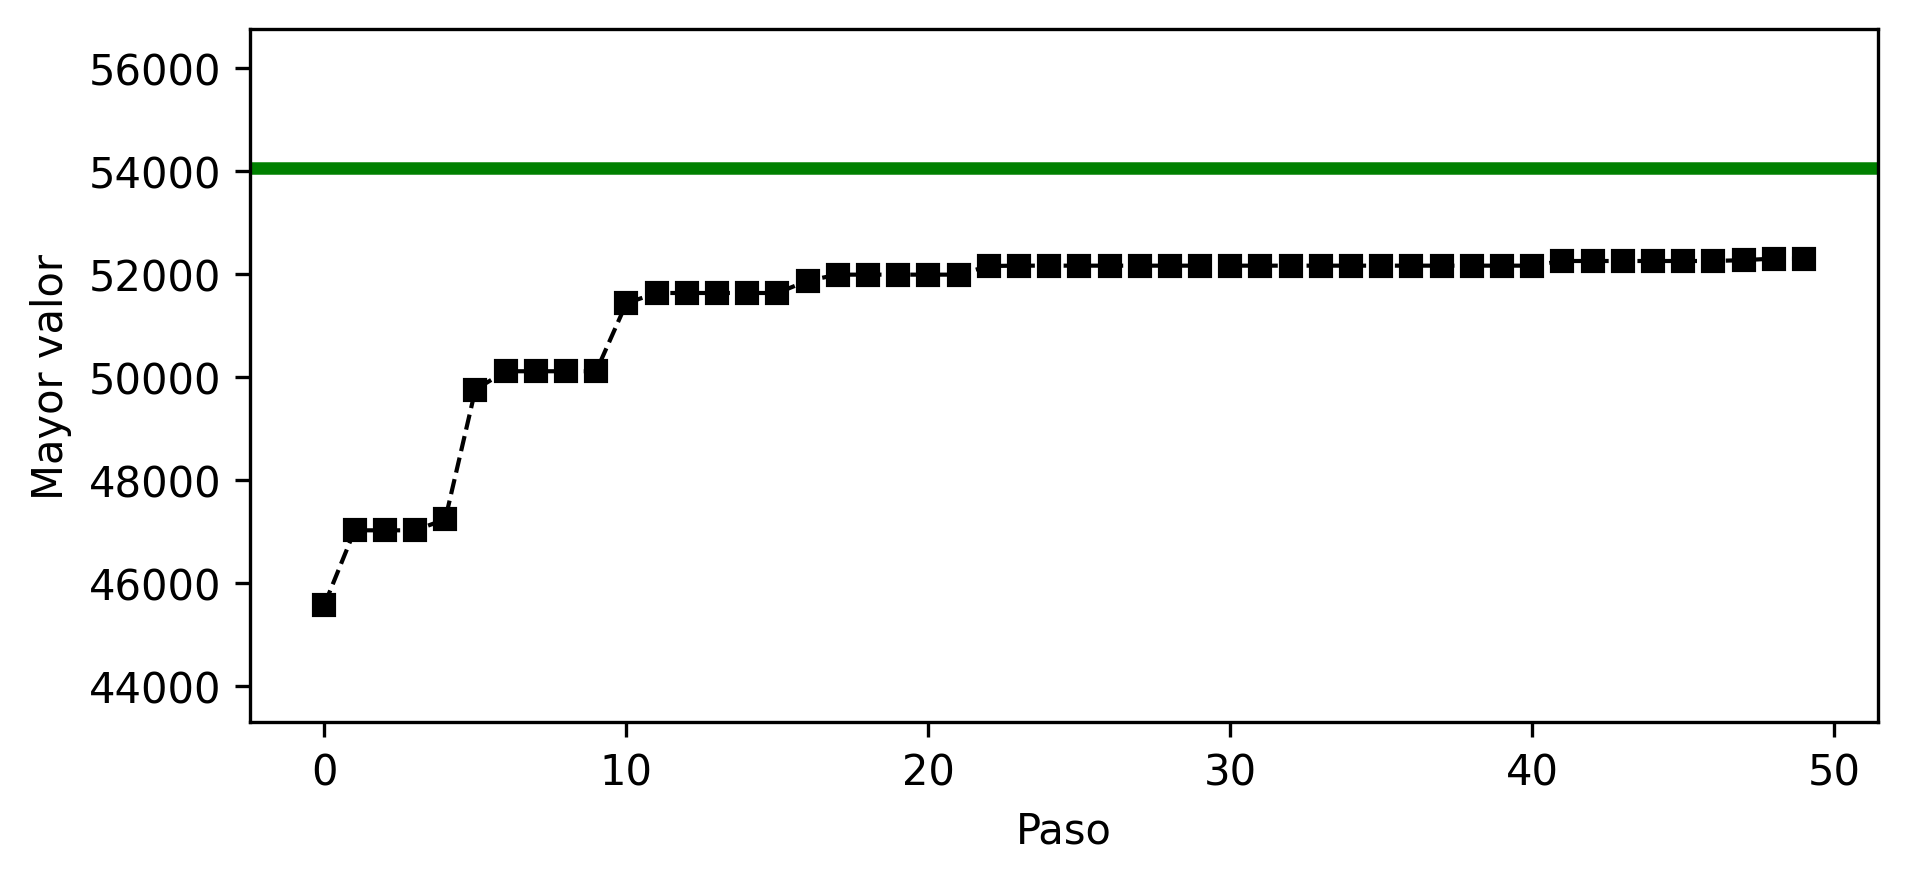
\includegraphics[width=\linewidth]{p300.png}
           \caption{Instancia 1}
           \label{fig:westminster_lateral}
        \end{subfigure}
          \begin{subfigure}[b]{0.49\linewidth}
           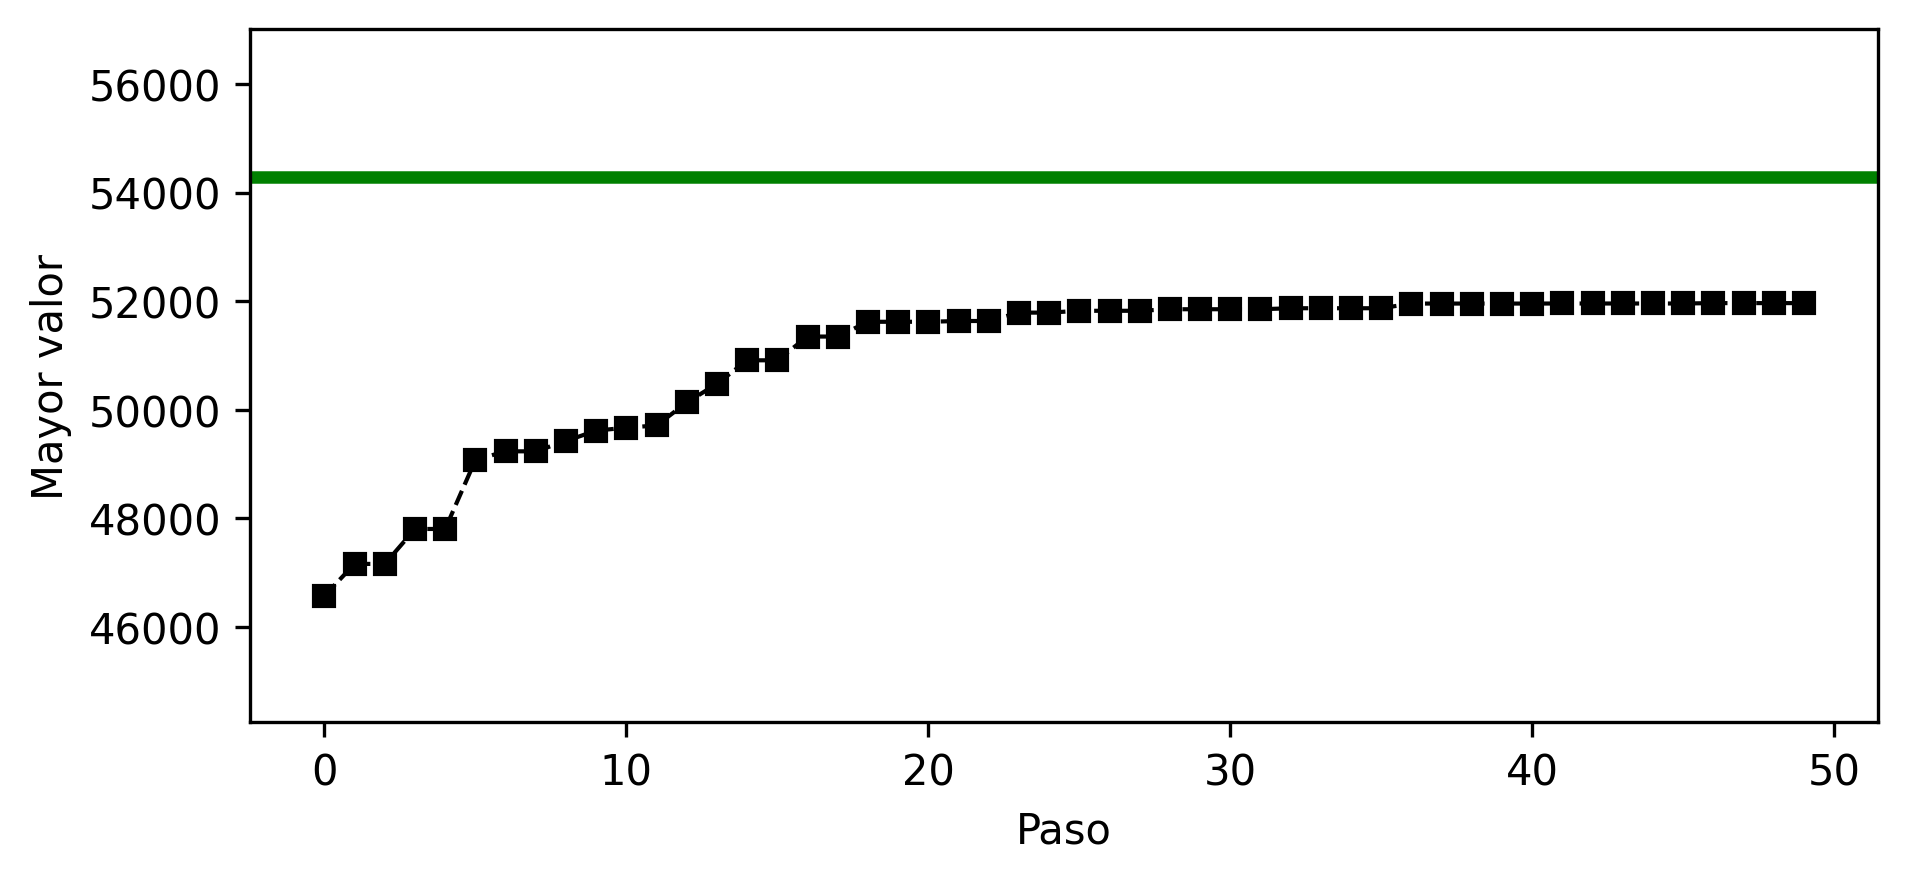
\includegraphics[width=\linewidth]{p300 i 2.png}
           \caption{Instancia 2}
           \label{fig:westminster_lateral}
        \end{subfigure}
       \begin{subfigure}[b]{0.49\linewidth}
           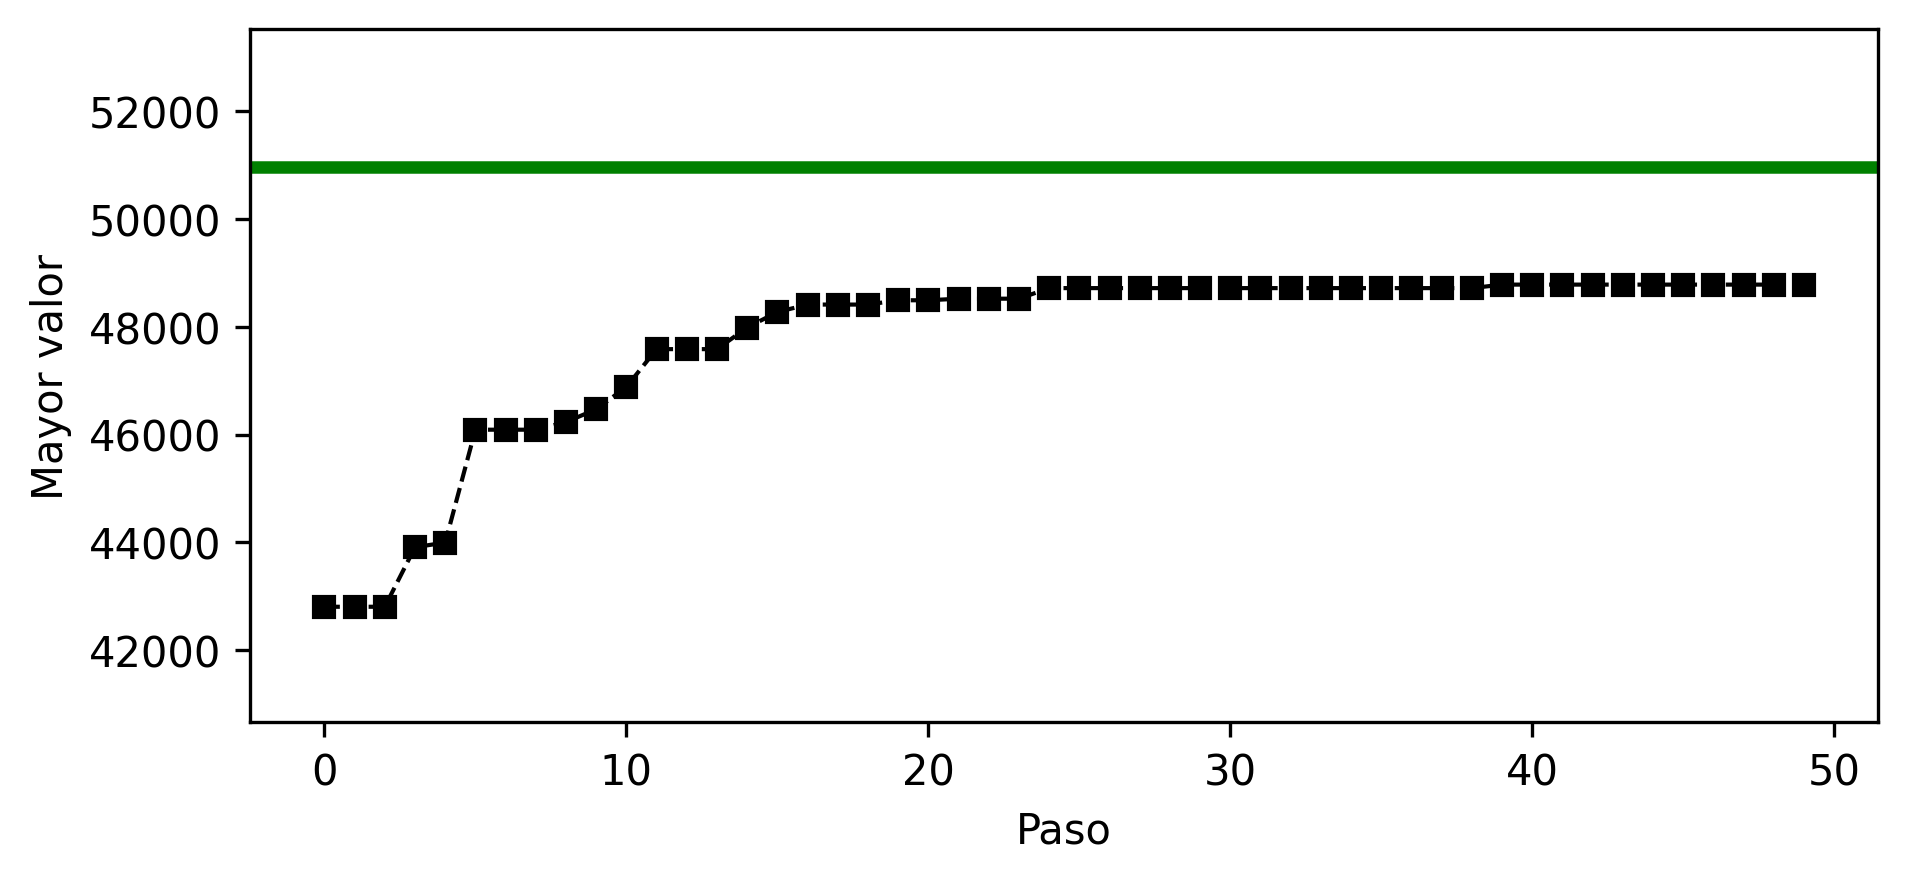
\includegraphics[width=\linewidth]{p300 i 3.png}
           \caption{Instancia 3}
           \label{fig:westminster_lateral}
        \end{subfigure}   
        \caption{3 instancias para n=300}
        \label{fig:westminster}
\end{figure}

\begin{figure}[H]
       \centering
       \begin{subfigure}[b]{0.49\linewidth}
           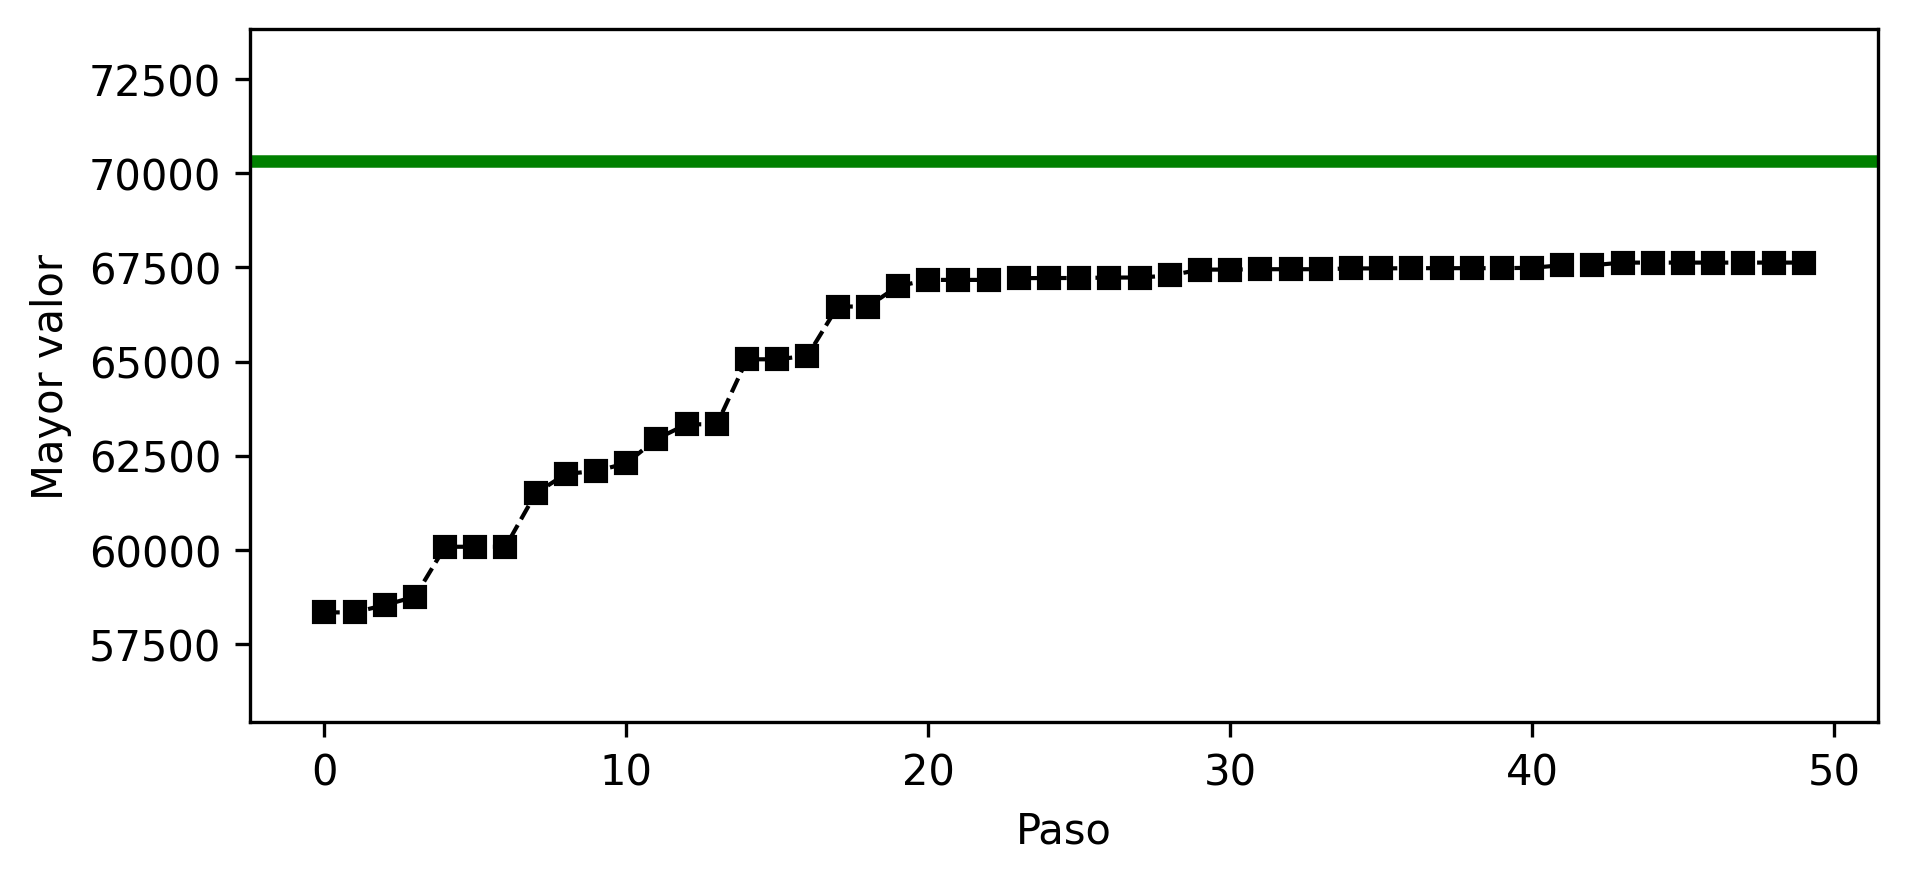
\includegraphics[width=\linewidth]{p400.png}
           \caption{Instancia 1}
           \label{fig:westminster_lateral}
        \end{subfigure}
          \begin{subfigure}[b]{0.49\linewidth}
           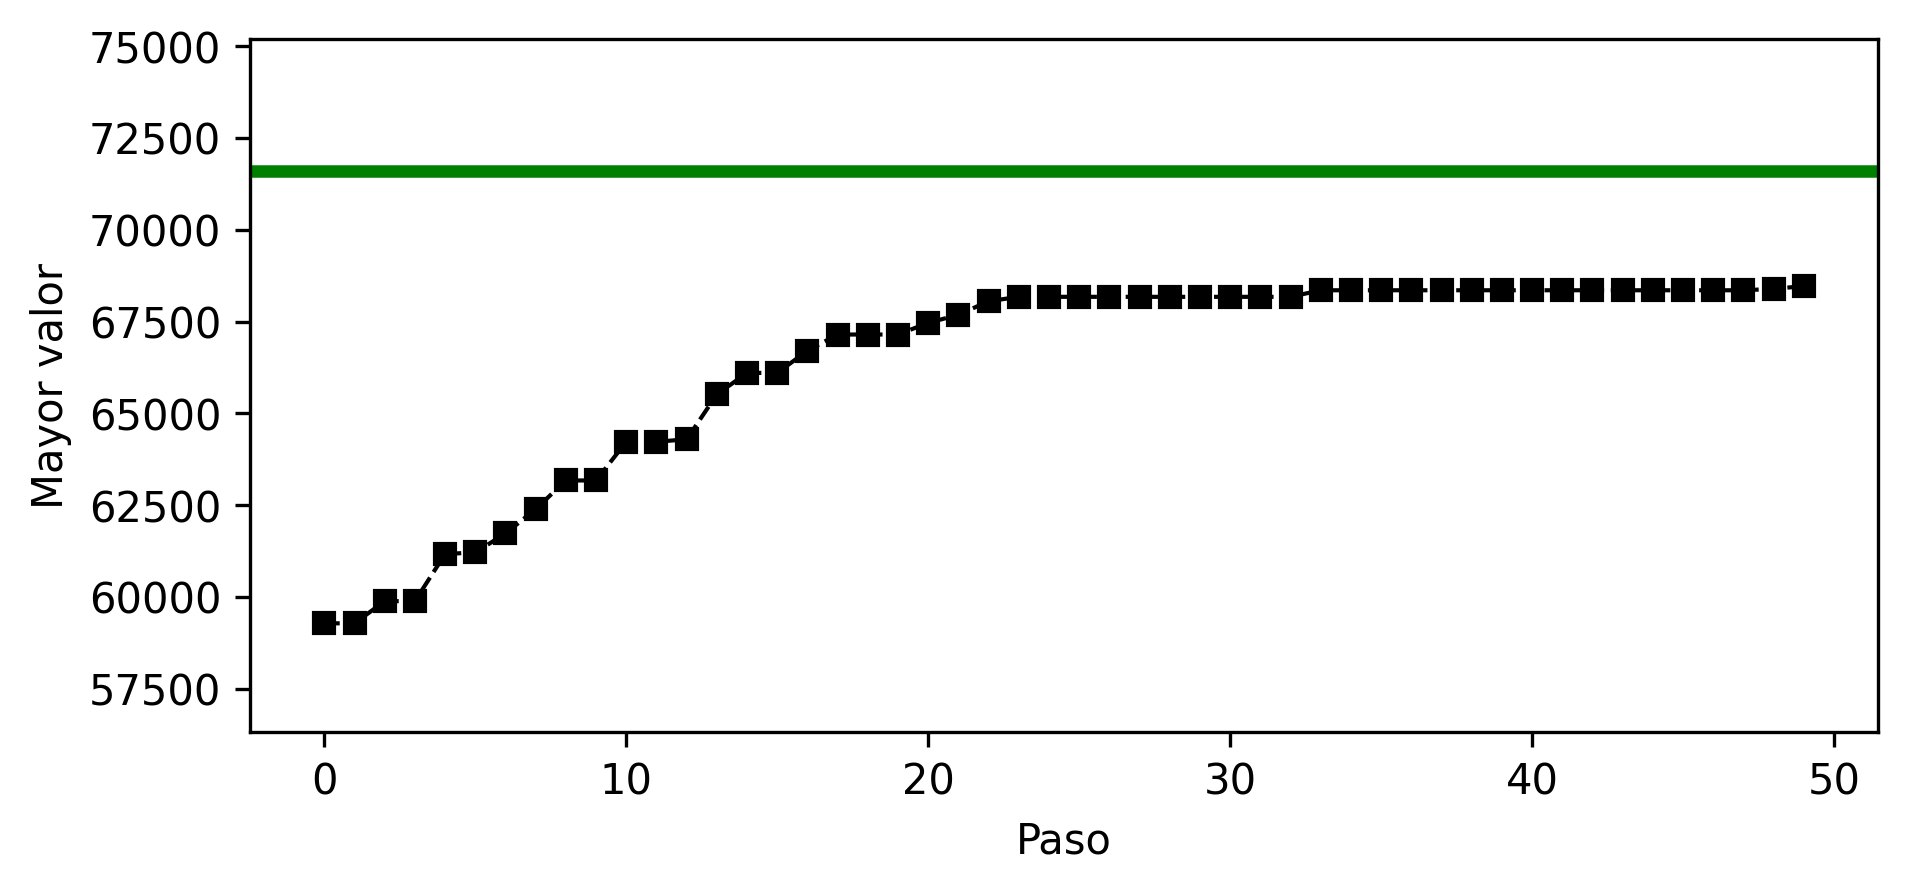
\includegraphics[width=\linewidth]{p400 i 2.png}
           \caption{Instancia 2}
           \label{fig:westminster_lateral}
        \end{subfigure}
       \begin{subfigure}[b]{0.49\linewidth}
           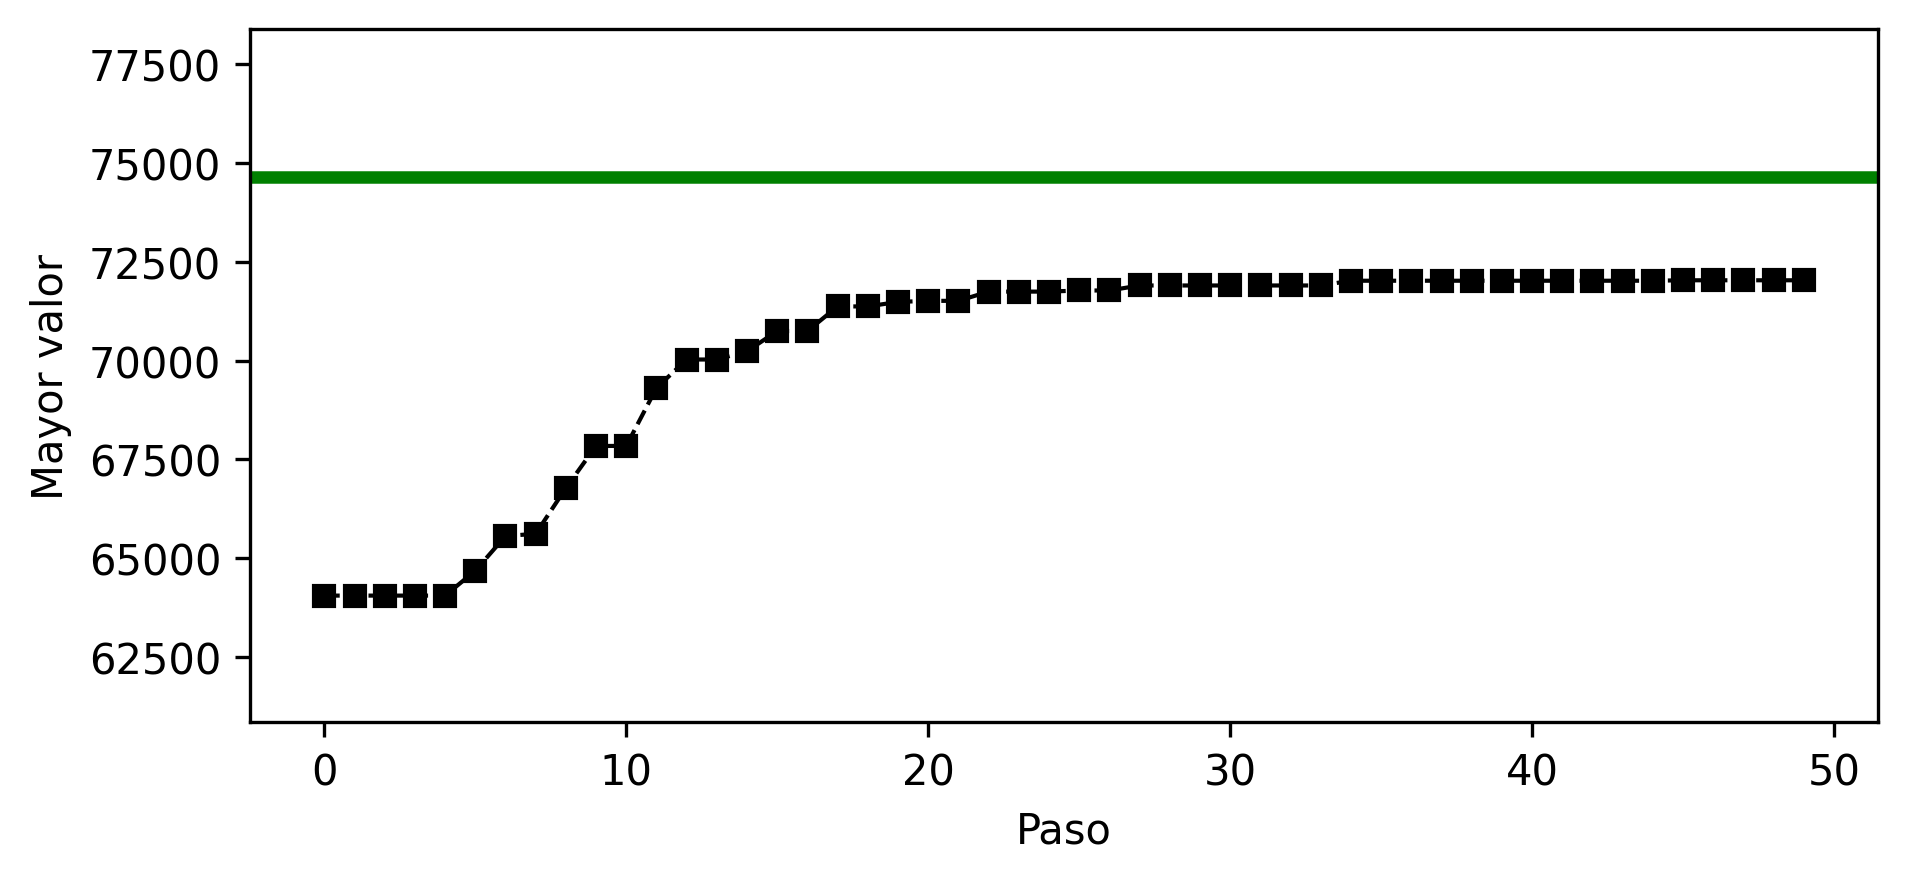
\includegraphics[width=\linewidth]{p400 i 3.png}
           \caption{Instancia 3}
           \label{fig:westminster_lateral}
        \end{subfigure}   
        \caption{3 instancias para n=400}
        \label{fig:westminster}
\end{figure}


\newpage
\section{Conclusi\'on}

Como se puede ver en las gr\'aficas, existe una l\'inea verde la cual nos refleja el valor m\'aximo de las 3 condiciones iniciales con respecto a las cantidades de n utilizadas en cada una de ellas \cite {yo}. Los valores \'optimos ser\'ian los que tocan la l\'inea verde en los valores de n indicados al pie de las gr\'aficas, sin embargo, en esta simulaci\'on no se alcanz\'o este punto posiblemente por la cantidad de objetos o por la capacidad del CPU para procesar los datos, aunque se puede decir que las 3 instancias muestran resultados muy similares.

\bibliography{tareadiez}
\bibliographystyle{unsrtnat}

\end{document}
